\documentclass[12pt]{article}
\usepackage{amsmath,amssymb,amsthm}
\usepackage[makeroom]{cancel}
\usepackage{graphicx}
\usepackage{color, colortbl}
\definecolor{LightRed}{rgb}{1.0,0.78,0.78}
\usepackage{listings}
\usepackage[final]{pdfpages}
\begin{document}
\lstset{breaklines=true,xleftmargin=-50pt}

\title{Deliverable 4---Query Design}
\date{\today}
\author{Galen Cochrane, Jonathan Glines, Nicholas Harrison }

\maketitle

\tableofcontents

\newpage

\section{Database Initialization}
\lstinputlisting[language=SQL,title=./init.sql]{./init.sql}

\section{Database Sample Data}
\lstinputlisting[language=SQL,title=values/accessory.sql]{values/accessory.sql}
\lstinputlisting[language=SQL,title=values/customer.sql]{values/customer.sql}
\lstinputlisting[language=SQL,title=values/equipment.sql]{values/equipment.sql}
\lstinputlisting[language=SQL,title=values/equipment\_type.sql]{values/equipment_type.sql}
\lstinputlisting[language=SQL,title=values/equipped\_with.sql]{values/equipped_with.sql}
\lstinputlisting[language=SQL,title=values/line\_item\_accessory.sql]{values/line_item_accessory.sql}
\lstinputlisting[language=SQL,title=values/line\_item\_equipment.sql]{values/line_item_equipment.sql}
\lstinputlisting[language=SQL,title=values/order.sql]{values/order.sql}
\lstinputlisting[language=SQL,title=values/rental\_contract.sql]{values/rental_contract.sql}
\lstinputlisting[language=SQL,title=values/rental\_history.sql]{values/rental_history.sql}
\lstinputlisting[language=SQL,title=values/rental\_item.sql]{values/rental_item.sql}
\lstinputlisting[language=SQL,title=values/reservation.sql]{values/reservation.sql}
\lstinputlisting[language=SQL,title=values/reservation\_item.sql]{values/reservation_item.sql}
\lstinputlisting[language=SQL,title=values/supplier.sql]{values/supplier.sql}

\section{Queries}
\subsection*{Query 1}
List the equipment ID, due date, and status for all equipment that is currently
rented.
\lstinputlisting[language=SQL,title=./queries/query01.sql]{./queries/query01.sql}
\subsection*{Query 2}
List all equipment types whose description ends with ``kayak".
\lstinputlisting[language=SQL,title=./queries/query02.sql]{./queries/query02.sql}
\subsection*{Query 3}
List the customer name, equipment type, equipment id, and scheduled return date
for all equipment rented (picked up) on October 9, 2015.
\lstinputlisting[language=SQL,title=./queries/query03.sql]{./queries/query03.sql}
\subsection*{Query 4}
List all rental incident reports (customer id, customer name, date, problem
description, amount owed) associated with a specified customer.
\lstinputlisting[language=SQL,title=./queries/query04.sql]{./queries/query04.sql}
\subsection*{Query 5 (a)}
List each equipment type and the total number of rentals from that category.
\lstinputlisting[language=SQL,title=./queries/query05a.sql]{./queries/query05a.sql}
\subsection*{Query 5 (b)}
List the type of equipment and total number of rentals for the equipment type
that was rented most often.
\lstinputlisting[language=SQL,title=./queries/query05b.sql]{./queries/query05b.sql}
\subsection*{Query 6}
List all equipment types and number of suppliers for those equipment types that
were supplied by multiple suppliers.
\lstinputlisting[language=SQL,title=./queries/query06.sql]{./queries/query06.sql}
\subsection*{Query 7}
Given an equipment type (e.g., Canoe), indicate the description and the number
of items that are available to be rented (in stock).
\lstinputlisting[language=SQL,title=./queries/query07.sql]{./queries/query07.sql}
\subsection*{Query 8}
List the equipment id, equipment type, and status of all rentals that are
overdue.
\lstinputlisting[language=SQL,title=./queries/query08.sql]{./queries/query08.sql}
\subsection*{Query 9}
List the total amount owed for all incident reports in the rental history
table.
\lstinputlisting[language=SQL,title=./queries/query09.sql]{./queries/query09.sql}
\subsection*{Query 10}
Count teh number of reservations that are scheduled to be picked up during the weekend of May 14 \& 15, 2016.
\lstinputlisting[language=SQL,title=./queries/query10.sql]{./queries/query10.sql}
\subsection*{Query 11}
Show the equipment type id, equipment type description, and average days rented
for all types of equipment on a type-by-type basis.
\lstinputlisting[language=SQL,title=./queries/query11.sql]{./queries/query11.sql}
\subsection*{Query 12}
List supplier number and supplier name for all suppliers for which there are no
current orders. Sort the list in ascending order by supplier name.
\lstinputlisting[language=SQL,title=./queries/query12.sql]{./queries/query12.sql}

\section{Output (All Queries)}
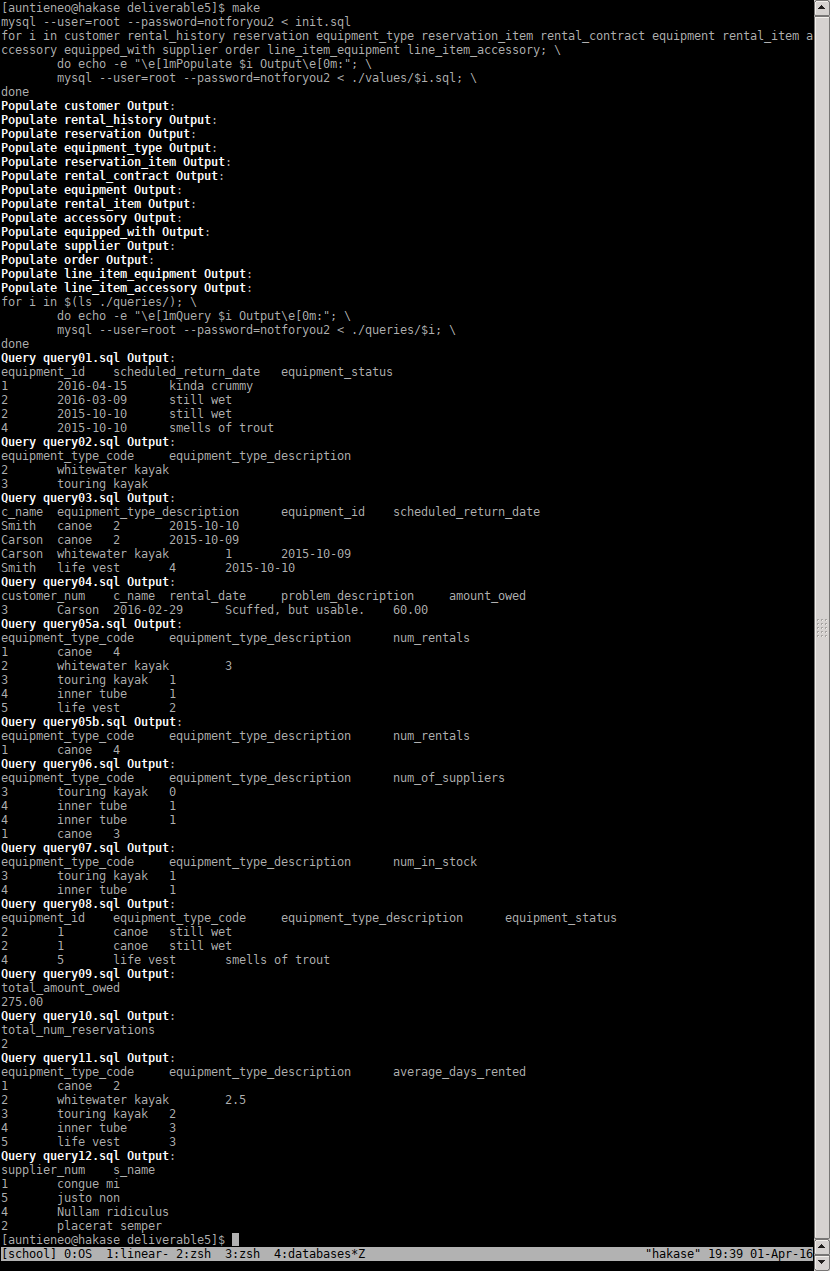
\includegraphics[scale=0.45]{./screenshots/deliverable5output.png}

\end{document}
